\section{Proof of Proposition \ref{lem:copulavalid}}
\label{app:proof}
\begin{prop*}[Validity of CopulaCPTS]
The confidence region provided by CopulaCPTS (algorithm \ref{alg:cpts}) \edit{is} valid. i.e. $ \edit{\Prob}[\: \forall h \in \{1,\ldots, k\}, \: \mathbf{y}_{t+h} \in \Gamma^{1-\alpha}_h\: ] \geq 1-\alpha$.
\end{prop*}

\begin{proof}
We assume that our estimation of $C_{\text{empirical}}$ is accurate. Via search, we found  $\mathbf{u^*} = (\hat{F}_1(s^*_1), \ldots, \hat{F}_t(s^*_k))$ such that
\begin{align}
    C_{\text{empirical}} (\mathbf{u^*}) = \displaystyle \mathop{\mathbb{E}}_\textbf{u}  \prod_{t=1}^{k}  \mathbbm{1}_{\mathbf{u}^*_t <\mathbf{u}_t} \geq 1-\alpha
\end{align}
Let $(\mathbf{x}_{1:t}^{n+1}, \mathbf{y}_{t+1:t+h}^{n+1}) \sim \mathbf{X}\times \mathbf{Y}$ be a new data point. Denote $\hat{\mathbf{y}} = \hat{f}(\mathbf{x}_{1:t}^{n+1})$, the forecast given by the trained model. Because the $\hat{F}_h$ functions and $C_{\text{empirical}}$ are monotonously increasing, we have:
\begin{align*}
    P[\: \forall h \in \{1,\ldots, k\}, \: \mathbf{y}_{t+h} \in \Gamma^{1-\alpha}_h\: ] 
    &= C(\hat{F}_1(s^{n+1}_1), \ldots, \hat{F}_k(s^{n+1}_k))\\
    &\geq  C( \hat{F}_1(s^*_1), \ldots, \hat{F}_k(s^*_k)) \\
    &\geq 1-\alpha
\end{align*} 
\end{proof}


\section{Additional Algorithm Details}

\subsection{Upper and Lower bounds for Copulas}
To provide a better understanding of the properties of Copulas, consider the Frechet-Hoeffding Bounds (Theorem \ref{lem:bounds}). In fact, the Frechet-Hoeffding upper- and lower- bounds are both copulas. The lower bound is percisely the Bonferroni correction used in \cite{Schaar2021conformaltime} - therefore by estimating the copula more precisely instead of using a lower bound, we have a guaranteed efficiency improvement for the confidence region. 

%Copulas can be parametric or non-parametric; the Gaussian copula, for example, is used for pricing in financial markets \cite{Haugh2016copula}. 

\begin{theorem}[The Frechet-Hoeffding Bounds]
Consider a copula $C(u_1, \ldots, u_k)$. Then
\[
\max{\{1-k+\sum_{i=1}^k u_i, 0\} } \leq C(u_1, \ldots, u_k) \leq \min{ \{u_1, \ldots, u_k \}}
\]
\label{lem:bounds}
\end{theorem}

\subsection{Numerical optimization with SGD for search}
The empirical inverse CDF modeled the same way as Equation \ref{eq:cdf} is the same as the empirical quantile estimation (Equation \ref{eq:quantile}).
\begin{equation}
    \hat{F}^{-1}(p) := \inf\{s: (\frac{1}{|D_{cal}|} \sum_{z^i \in D_{cal} } \mathbbm{1}_{A(z, \hat{f}) \leq s}) \geq p \}
    \label{eq:inverse_cdf}
\end{equation}


We find the optimal $s_h^*$ in Equation \ref{eq:search} and Algorithm \ref{alg:cpts} by minimizing the following loss: 
\[
\gL(s_1, \ldots, s_k) = \frac{1}{n-m} \sum_{i=m+1}^{n} \prod_{h=1}^k \mathbbm{1}\left[ \mathbf{u}^i_h < \hat{F}_h^{-1}(s_h) \right] - (1-\alpha) 
\]
We use the Adam optimizer and optimize for 500 steps. An alternative and faster way of search is to assume $s_1 = s_2 = \cdots = s_k$ which simplifies the search from exponential time to constant time. 

\subsection{Autoregressive prediction}
\label{lab:autoregressive}
In the context of this paper to forecast autoregressively is given input $\textbf{x}_{1:t}$ and a $k$ step forecasting model $\hat{f}$, perform prediction

\begin{align*}
    \hat{\textbf{y}}_{t+1:t+k} &= \hat{f}(\textbf{x}_{1:t}) \\
    \hat{\textbf{y}}_{t+2:t+k+1} &= \hat{f}(\textbf{x}_{2:t},  \hat{\textbf{y}}_{t+1}) \\
    & \cdots
\end{align*}

until all $k'$ time steps are predicted. 

We now provide a toy scenario to illustrate when re-estimating the copula is necessary and improves validity. Consider a time series of three time steps $t_0, t_1, t_2$. The two scenarios are illustrated in Figure \ref{fig:ar}. In both scenarios the mean and variance of all timeseps are $0$ and $1$ respectively.  In scenario (a), $t_0 = t_1$ and hence their covariance is $1$. The copula estimated on $t_0$ and $t_1$ is $C_{0:1}(F(t_0), F(t_1)) = F(t_0) = F(t_1)$.  This copula will significantly underestimate the confidence region of  $t_2$ where its covariance with $t_1$ is $-1$. In fact the coverage of $C_{0:1}(F_1(t_1), F_2(t_2)) =0.74 $. On the other hand, (b) illustrates a scenario where the copula for any 2 consecutive time series remain the same $C_0=C_1$. In this case, applying $C_0$ directly to forecast $C_1$ achieves precisely 90\% coverage.


\begin{figure}[h!]
\centering
\begin{subfigure}[b]{0.45\linewidth}
  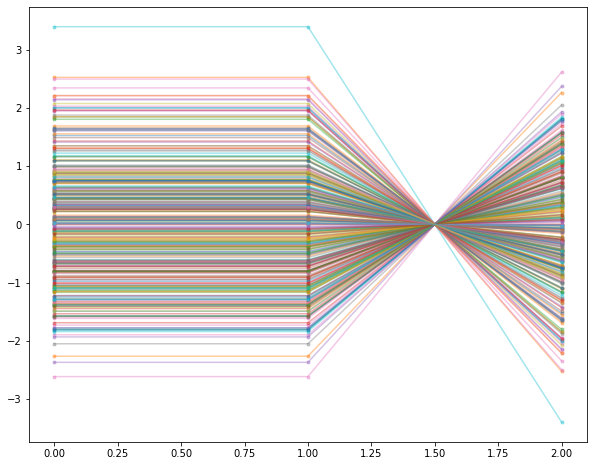
\includegraphics[width=\linewidth]{copula/figs/appscene1.png}
  \caption{Time steps 0 and 1 are positively correlated while 1 and 2 are negatively correlated}
  \label{fig:cal001}
\end{subfigure}
\hspace{0.8em}
\begin{subfigure}[b]{0.45\linewidth}
  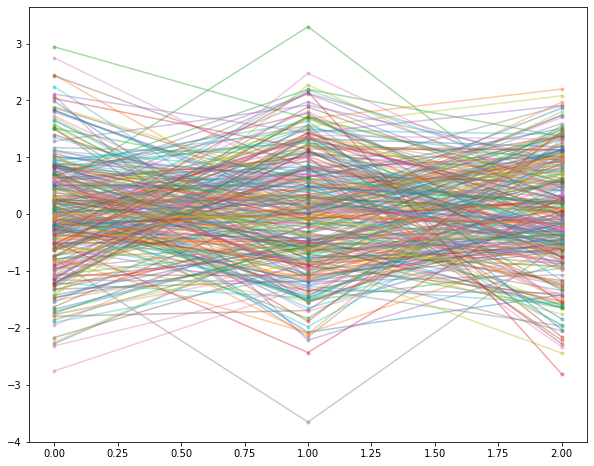
\includegraphics[width=\linewidth]{copula/figs/appscene2.png}
  \caption{Stationary time series where each time steps are uncorrelated}
  \label{fig:cal002}
\end{subfigure}%
\caption{Two scenarios to illustrate the autoregressive case}
\label{fig:ar}
\end{figure}



\section{Experiment Details and additional results}
\label{app:exp_details}

\subsection{Underlying forecasting models}

\edit{
\paragraph{Particle Dataset}
The underlying forecasting model for the particle experiments is an 1-layer LSTM network with embedding size $=24$. The hidden state is then passed through a linear network  to forecast the timesteps concurrently (output has dimension $k \times d_y$).  We train the model for 150 epochs with batch size 128. Hyperparameters of the network are selected through a model search by performance on a 5-fold cross validation split of the dataset. The architecture and hyperparameters are shared for all baselines and CopulaCPTS in Table 1.

\paragraph{Drone} For the drone trajectory forecasting task, we use he same LSTM forecasting network as the particle dataset, but with hidden size increased to 128.  We train the model for 500 epochs with batch size 128. The same architecture and hyperparameters are shared for all baselines and CopulaCPTS reported in Table 1. 

\paragraph{Covid-19} The base forecasting model for Covid-19 dataset is the same as the synthetic datasets, with hidden size $=128$ and were trained for 150 epochs with batch size 128. The same architecture and hyperparameters are shared for all baselines and CopulaCPTS reported in Table 1. 

\paragraph{Argoverse} As highlighted in the main text, we utilize a state-of-the-art prediction algorithm LaneGCN \cite{liang2020learning} as the underlying forcaster model for CF-RNN and Copula-RNN. We refer the readers to their paper and code base for model details. The architecture of the RNN network used for MC-Dropout and BJRNN is an Encoder-Decoder network. Both the encode and decoder contains a LSTM layer with encoding size 8 and hidden size 16. We chose this architecture because the is part of the official Argoverse baselines (\texttt{https://github.com/jagjeet-singh/argoverse-forecasting}) and demonstrates competitive performance.  
}


\subsection{COVID-19 Dataset}
The COVID-19 dataset is downloaded directly from the official UK government website \texttt{https://coronavirus.data.gov.uk/details/download} by selecting \textit{region} for area type and \textit{newCasesByPublishDate} for metric. There are in total 380 regions and over 500 days of data, depending when it is downloaded. We selected 150-day time series from the collection to construct our dataset.


\subsection{Calibration and Efficiency chart for COVID-19}
Figure \ref{fig:covid-day} shows comparison of calibration and efficiency for the daily new COVID 19 cases forecasting. 
\begin{figure}[h!]
    \centering
    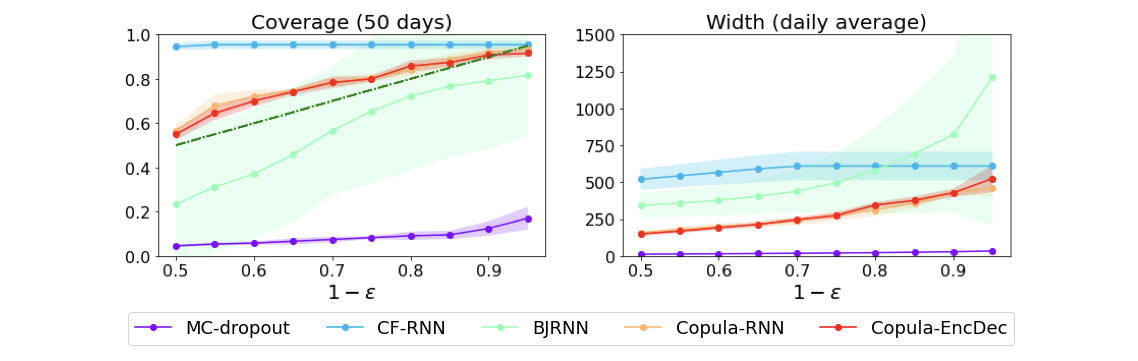
\includegraphics[width=\linewidth]{copula/figs/covid_cov_daily.jpeg}
    \caption{Calibration and efficiency comparison on different $\epsilon$ level for COVID-19 Daily Forecasts. The copula methods (orange and red lines) are more calibrated (coinciding with the green doted line) and sharp (low width) compared to baselines.}
    \label{fig:covid-day}
\end{figure}

To see if the daily fluctuation due to testing behaviour disrupts other method, we also ran the same experiment on weekly aggregated new cases forecast. We take 14 weeks of data as input and output forecasts for the next 6 weeks. The results are illustrated in Figure \ref{fig:covid-week}. The weekly forecasting scenario gives us similar insights as the daily forecasts. 

\begin{figure}[h!]
    \centering
    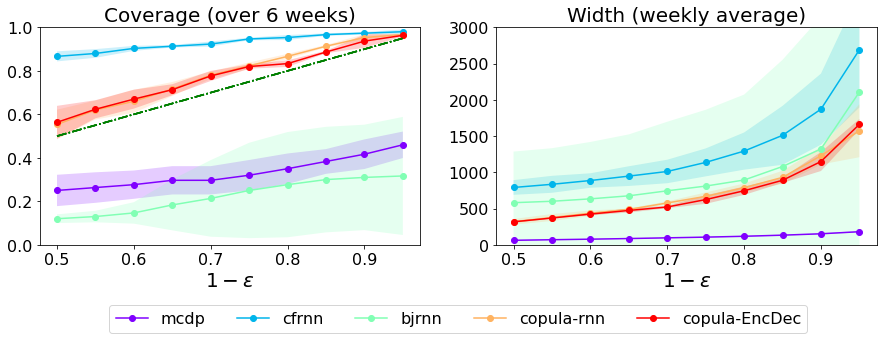
\includegraphics[width=0.8\linewidth]{copula/figs/covidcoverage.png}
    \caption{Covid Weekly Forecasts}
    \label{fig:covid-week}
\end{figure}

\subsection{Argoverse}
The Argoverse autonomous vehicle dataset contains 205,942 samples, consisting of diverse driving scenarios from Miami and Pittsburgh.  The data can be downloaded from the official Argoverse dataset website. We split 90/10 into a training set and validation set of size 185,348 and 20,594 respectively. The official validation set of size 39,472 is used for testing and reporting performance. We preprocess the scenes to filter out incomplete trajectories and cap the number of vehicles modeled to 60. If there are less than 60 cars in the scenario, we insert dummy cars into them to achieve consistent car numbers. For map information, we only include center lanes with lane directions as features. Similar to vehicles, we introduce dummy lane nodes into each scene to make lane numbers consistently equal to 650.

\subsection{Additional Experiment Results}
We present in figure 8 and 9  some qualitative results for uncertainty estimation.  

\edit{ To test how the effects of copulaCPTS compare with baseline on other base forecasters, we also include an encoder-decoder architecture with the same embedding size as the RNN models introduced in appendix C.1 for each dataset. The results are presented in Table \ref{tab:baselines}. We omit these results in the main text because we found that they do did not bring significant improvement to time series forecasting UQ. 

Table \ref{tab:horizon} compares model performance compared across different prediction horizons. We show that the advantage of our method is more pronounced for longer horizon forecasts. 

}

% ---------------------------------
% drone vis
% ---------------------------------


\begin{figure}[h]
\centering
\begin{subfigure}[b]{0.33\linewidth}
  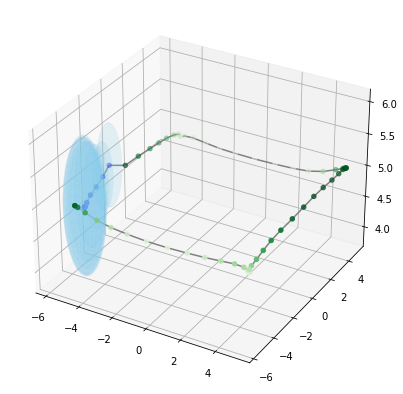
\includegraphics[width=\linewidth]{copula/figs/dronecopula.png}
  \caption{Copula-EncDec}
\end{subfigure}%
\begin{subfigure}[b]{0.33\linewidth}
  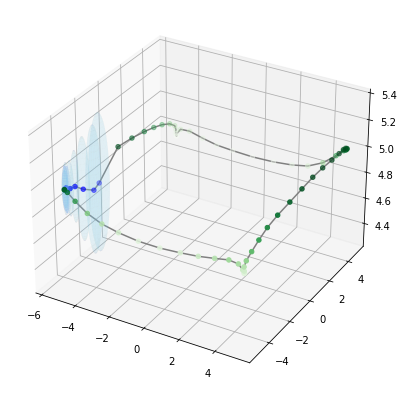
\includegraphics[width=\linewidth]{copula/figs/dronemcdp.png}
  \caption{MC Dropout}
\end{subfigure}%
\begin{subfigure}[b]{0.33\linewidth}
  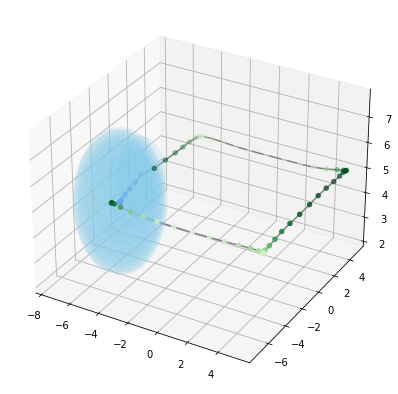
\includegraphics[width=\linewidth]{copula/figs/dronecf.png}
  \caption{CF-RNN}
\end{subfigure}
\caption{ $99\%$ Confidence region produced by three methods for the drone dataset. Copula methods (a) produces a more consistent, expanding cone of uncertainty compared to MC-Dropout (b) sharper one compared to CF-RNN (c). }
\label{fig:drone}
\end{figure}


\begin{figure*}[h!]
\centering
\begin{subfigure}{.245\textwidth}
  \centering
  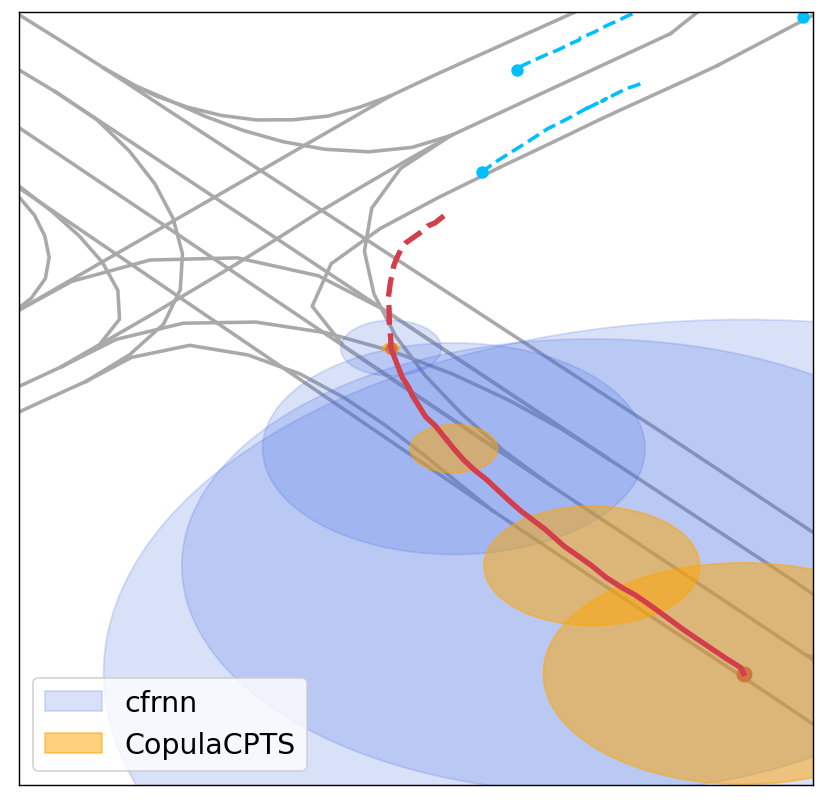
\includegraphics[width=.9\linewidth]{copula/figs/argoverse1.png}
\end{subfigure}%
\begin{subfigure}{.245\textwidth}
  \centering
  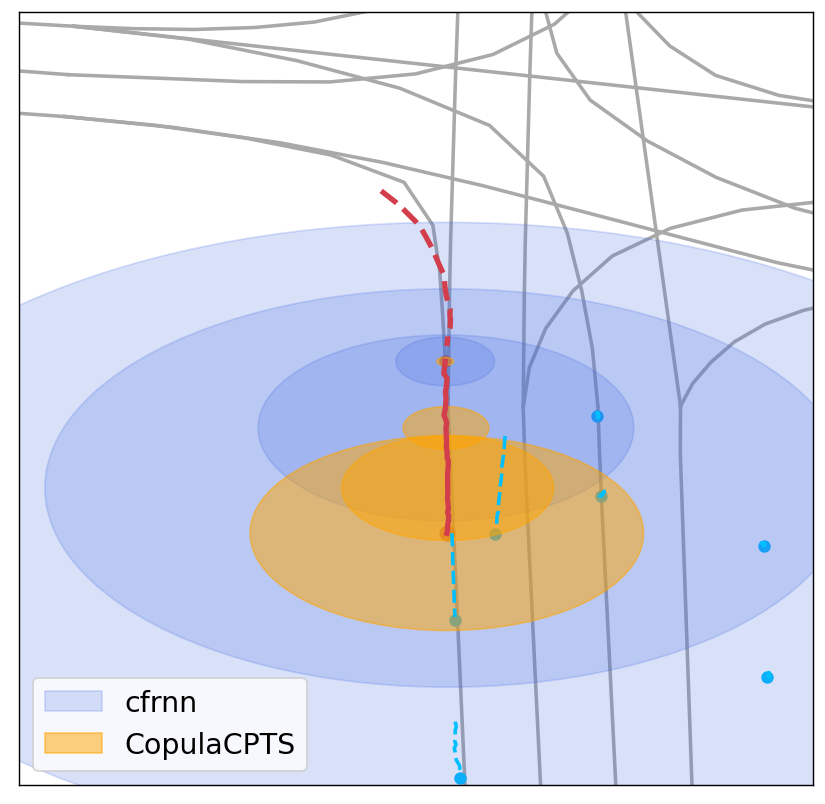
\includegraphics[width=.9\linewidth]{copula/figs/argoverse2.png}
\end{subfigure}
\begin{subfigure}{.245\textwidth}
  \centering
  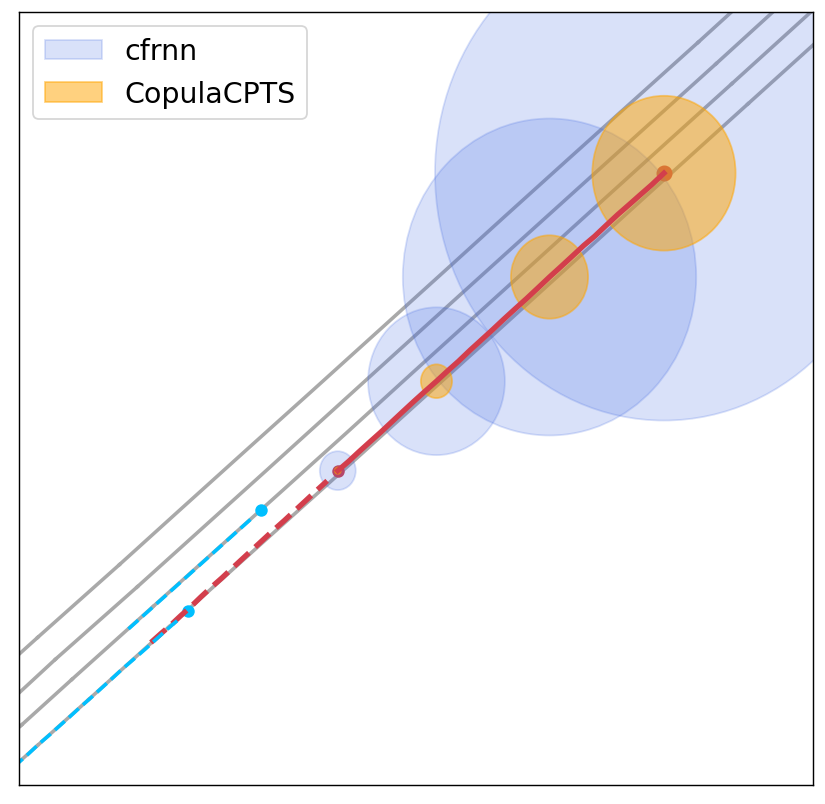
\includegraphics[width=\linewidth]{copula/figs/argoverse3.png}
\end{subfigure}%
\begin{subfigure}{.245\textwidth}
  \centering
  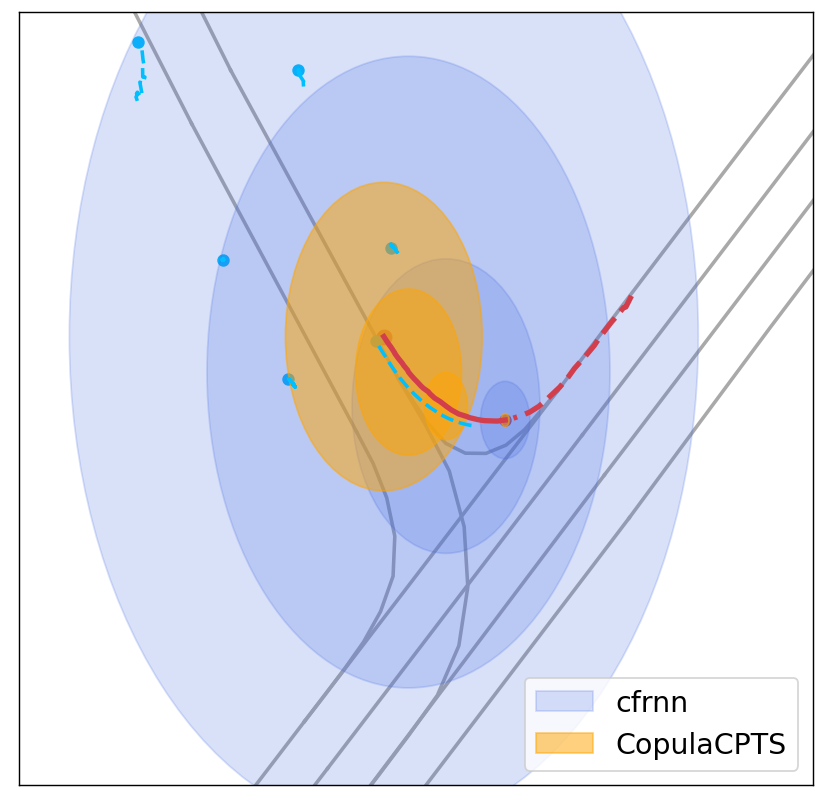
\includegraphics[width=\linewidth]{copula/figs/argoverse4.png}
\end{subfigure}
\caption{Illustrations for confidence regions given by CF-RNN (blue) and CopulaCPTS (orange) in at time steps 0, 10, 20, and 30. Note that in order to achieve 90\% coverage, the regions are larger than needed, especially in straight-lane cases like the middle two. Using copulas to couple together time steps results in a much smaller region, while achieving similarly good coverage.}
\label{fig:argo}
\end{figure*}



% ---------------------------------
% Big big master table
% ---------------------------------
\begin{table*}
\centering
\begin{tabular}{ c | c c  | c c  } 
 \toprule
  \multicolumn{5}{c}{Particle Simulation ($\sigma=.01$)} \\
    \midrule
     & Coverage (90\%) & Area (90\%)   & Coverage (99\%)  & Area (99\%)  \\
  \midrule
    MC-dropout &  63.9 \plusminus 16.1  &  0.81 \plusminus 0.05  &  73.1 \plusminus 14.2  &  1.14 \plusminus 0.07  \\ 
BJRNN &  98.9 \plusminus 0.2  &  2.24 \plusminus 0.59  &   100 \plusminus 0.0  &  3.75 \plusminus 0.71  \\ 
CF-RNN &  97.0 \plusminus 2.3  &  3.13 \plusminus 3.24  &   100  \plusminus 0.21   &   4.34 \plusminus 1.19   \\ 
Copula-RNN &  91.5 \plusminus 2.1  &  \textbf{1.06} \plusminus 0.36  &  97.4 \plusminus 2.4  &  4.47 \plusminus 1.48  \\ 
Copula-EncDec &  \textbf{90.2} \plusminus 2.3  &  1.19 \plusminus 0.17  &  \textbf{99.6} \plusminus 0.7  &  \textbf{1.83} \plusminus 0.09  \\ 
    \midrule
  \multicolumn{5}{c}{Particle Simulation ($\sigma=.05$)} \\
  \midrule 
  & Coverage (90\%) & Area (90\%)   & Coverage (99\%)  & Area (99\%)  \\
  \midrule
  MC-dropout &  16.1 \plusminus 4.3  &  0.79 \plusminus 0.02  &  33.9 \plusminus 5.1  &  2.12 \plusminus 0.03  \\ 
BJRNN &  100.0 \plusminus 0.0  &  12.13 \plusminus 0.39  &  100.0 \plusminus 0.0  &  15.43 \plusminus 0.85  \\ 
CF-RNN &  94.5 \plusminus 1.5  &  5.79 \plusminus 0.51 &  99.8 \plusminus 2.2  &  19.21 \plusminus 8.19  \\ 
Copula-RNN &  \textbf{90.3} \plusminus 0.7  &  4.50 \plusminus 0.07  &  \textbf{99.1} \plusminus 0.8  &  12.82 \plusminus 3.98  \\ 
Copula-EncDec & 91.4 \plusminus 1.1  & \textbf{4.40} \plusminus 0.15  &  98.7 \plusminus 0.1  & \textbf{9.31} \plusminus 1.97  \\ 
    \midrule
  \multicolumn{5}{c}{Drone Simulation ($\sigma=.02$)}\\
  \midrule
   & Coverage (90\%) & Area (90\%)   & Coverage (99\%)  & Area (99\%)  \\
  \midrule
  MC-dropout &  84.5 \plusminus 10.8  &  9.64 \plusminus 2.13 &  90.0 \plusminus 7.8  &  16.02 \plusminus 3.62 \\ 
BJRNN &  90.8 \plusminus 2.8  &  49.57 \plusminus 3.77 &  100.0 \plusminus 4.0  &  65.77 \plusminus 4.56 \\ 
CF-RNN &  91.6 \plusminus 9.2  &  32.18 \plusminus 13.66 &  100.0 \plusminus 0.0  &  36.79 \plusminus 14.03 \\ 
CF-EncDec &  100.0 \plusminus 0.0  &  21.83 \plusminus 26.29 &  100.0 \plusminus 0.0  &  25.03 \plusminus 12.53 \\ 
Copula-RNN &  \textbf{90.0} \plusminus 1.5  &  \textbf{16.52} \plusminus 15.08 &  \textbf{98.5} \plusminus 0.5  &  \textbf{21.48} \plusminus 8.91 \\ 
    \midrule
  \multicolumn{5}{c}{COVID-19 Daily Cases Dataset} \\
  \midrule
    & Coverage (90\%) & Area (90\%)   & Coverage (99\%)  & Area (99\%)  \\
  \midrule
 MC-dropout & 19.1 \plusminus 5.1 & 34.14 \plusminus 0.84  & 100.0 \plusminus 0.0 & 1106.57 \plusminus 25.41 \\
 BJRNN & 79.2 \plusminus 30.8 & 823.3 \plusminus 529.7 & 85.7 \plusminus 27.5 & 149187. \plusminus 51044. \\
 CF-RNN & 95.4 \plusminus 1.9 & 610.2 \plusminus 96.0 & 100.0 \plusminus 0.0 & 121435. \plusminus 26495. \\
 CF-EncDec & 91.7 \plusminus 1.4 & 570.3 \plusminus 22.1  & 100.0 \plusminus 0.0 & 108130. \plusminus 10889.\\
 Copula-RNN & 92.1 \plusminus 1.0 & \textbf{429.0} \plusminus 15.1 & 100.0 \plusminus 0.0 & 88962. \plusminus 9643.\\
 Copula-EncDec & \textbf{90.8} \plusminus 0.3 & 429.4 \plusminus 27.9 & 100.0 \plusminus 0.0 & \textbf{60852.} \plusminus 12263. \\
 \midrule  
  \multicolumn{5}{c}{Argoverse Trajectory Prediction Dataset} \\
 \midrule   
 & Coverage (90\%) & Area (90\%)   & Coverage (99\%)  & Area (99\%)  \\
  \midrule
MC-dropout & 27.9 \plusminus 3.1 & 127.6 \plusminus 20.9 &  31.5 \plusminus 3.9 & 242.1 \plusminus 54.0 \\
BJRNN & 92.6 \plusminus 9.2 & 880.8 \plusminus 156.2 & 100.0 \plusminus 0.0 & 3402.8 \plusminus 268. \\
CF-LaneGCN & 98.8 \plusminus 1.9 & 396.9 \plusminus 18.67 & 100. \plusminus 0.2 & 607.2 \plusminus 8.67 \\
Copula-LaneGCN & \textbf{90.4} \plusminus 0.3 & \textbf{126.8} \plusminus 12.22 & \textbf{99.1} \plusminus 0.4 & \textbf{324.1} \plusminus 42.22 \\
\bottomrule
\end{tabular}
\caption{Additional results. Copula methods achieves high level of calibration while producing sharper predictions regions. The sharpness gain is even more pronounced in at higher confidence levels (99\%), where we want the prediction region to be useful while remaining valid.} 
\label{tab:baselines}
\end{table*}

\begin{table*}[t]
\centering
\resizebox{\textwidth}{!}{
\begin{tabular}{ c | c c  | c c  | c c } 
 \toprule
  & \multicolumn{2}{c}{1 Step} & \multicolumn{2}{c}{5 Steps} &  \multicolumn{2}{c}{15 Steps}\\
 \midrule
Method & Coverage & Area & Coverage & Area & Coverage & Area \\
 \midrule
MC-Dropout & 97.8 \plusminus 2.0 & 0.4 \plusminus 0.04 & 88.0 \plusminus 7.0 & 0.69 \plusminus 0.25 & 52.3 \plusminus 1.4 & 0.94 \plusminus 0.2 \\ 
BJRNN & 45.3 \plusminus 39.4 & 0.27 \plusminus 0.18 & 97.7 \plusminus 2.1 & 2.69 \plusminus 1.79 & 95.5 \plusminus 2.8 & 19.99 \plusminus 4.83 \\ 
CF-RNN & 100.0 \plusminus 0.0 & \textbf{0.01} \plusminus 0.01 & 77.8 \plusminus 19.2 & 0.8 \plusminus 0.64 & 66.7 \plusminus 0.0 & 18.82 \plusminus 3.73 \\ 
CF-EncDec & 89.9 \plusminus 19.2 & \textbf{0.01} \plusminus 0.01 & 100.0 \plusminus 0.0 & 0.75 \plusminus 0.99 & 88.9 \plusminus 19.2 & 13.07 \plusminus 16.1 \\ 
Copula-RNN & 90.1 \plusminus 0.2 & \textbf{0.01} \plusminus 0.01 & 89.8 \plusminus 0.6 & \textbf{0.54} \plusminus 0.45 & \textbf{90.1} \plusminus 1.2 & 8.25 \plusminus 3.44 \\ 
Copula-EncDec & \textbf{90.0} \plusminus 0.3 & \textbf{0.01} \plusminus 0.0 & \textbf{90.3} \plusminus 0.6 & 0.67 \plusminus 1.01 & 90.5 \plusminus 0.5 & \textbf{7.13} \plusminus 9.5 \\ 
\bottomrule
\end{tabular}
}
\caption{Performance comparison across different horizons at 90\% confidence level on the drone simulation dataset. The improvement on efficiency is more pronounced when the horizon is longer.} 
\label{tab:horizon}
\end{table*}


\edit{\subsection{Study on $\alpha_h$ search}}

Figure \ref{fig:alpha} shows the $\alpha_h$ values for each $1-\alpha_h =\hat{F}_h(s_h^*)$ used in Copula CPTS as outlined in line 15 of Algorithm \ref{alg:cpts}. We present $\alpha_h$ values searched using two methods of searching, with dichotomy search for a constant $\alpha$ value for the horizon  as in \cite{messoudi2021copula}, and by stochastic gradient descent as outlined in section 4.2.  

The $\alpha_h$ values are an indicator of how interrelated the uncertainty between each time step are: Bonferroni Correction used in \cite{Schaar2021conformaltime}  (grey dotted line in Figure \ref{fig:alpha}) assumes that the time steps are independent, with CopulaCPTS we have lower $1 - \alpha_h$ levels while having valid coverage (blue and orange lines in Figure \ref{fig:alpha}). This shows that the uncertainty of the time steps are not independent, and we are able to utilize this dependency to shrink the confidence region and still maintaining the coverage guarantee.

Table \ref{tab:alphacomp} shows that there are no significant difference between coverage and area performance for the two search methods with in the scope of datasets we study in this paper. However, we want to highlight that SGD search is $O(n)$ complexity to optimization steps, regardless to the prediction horizon. SGD also allows for varying $\alpha_h$ which might be useful in some settings, for example capturing uncertainty spikes for some time steps as seen in the COVID-19 dataset of Figure \ref{fig:alpha}. Dichotomy search, on the other hand, is $O(n log(n))$ complexity to the search space depends on granularity, and will be $O(kn log(kn)$ if we want to search for varying $\alpha_h$.

\begin{table*}[h!]
    \centering
    \begin{tabular}{c|c c | c c}
        \toprule
         Dataset & \multicolumn{2}{c}{Coverage (90\%)} &  \multicolumn{2}{c}{Area} \\
         \midrule
         & Fixed $\alpha_h$ & Varying $\alpha_h$  &  Fixed $\alpha_h$ & Varying $\alpha_h$\\
         \midrule
         \midrule
         Particle ($\sigma = .01$) & 91.7 \plusminus 1.9   & 91.5 \plusminus 2.1 & 1.13 \plusminus 0.45  & 1.06 \plusminus 0.36 \\
                 \midrule
         Particle ($\sigma = .05$) & 92.1 \plusminus 1.3   & 90.3 \plusminus 0.7 & 4.89 \plusminus 0.05  & 4.50 \plusminus 0.07 \\
                 \midrule
        Drone &  90.3 \plusminus 0.5   & 90.0 \plusminus 1.5 & 15.92 \plusminus 1.98  & 16.52 \plusminus 7.08 \\
                \midrule
         Covid-19 &  92.9 \plusminus 0.1   & 92.1 \plusminus 1.0 & 498.44 \plusminus 6.36  & 429.0 \plusminus 15.1  \\
            \midrule
        Argoverse &  90.2 \plusminus 0.1   & 90.4 \plusminus 0.3 & 117.1 \plusminus 7.3  & 126.8 \plusminus 12.2 \\
        \bottomrule
    \end{tabular}
    \caption{Coverage and area comparison between stochastic search for fixed $\alpha_h$ and SGD for Varying $\alpha_h$. We do not see significant difference between the performance of two.}
    \label{tab:alphacomp}
\end{table*}

\begin{figure*}[h!]
\centering
\begin{subfigure}{.45\textwidth}
  \centering
  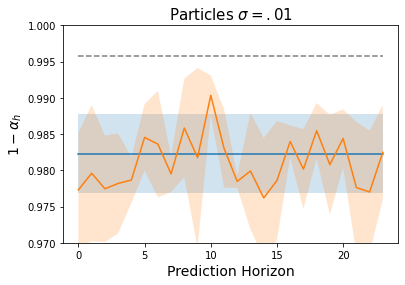
\includegraphics[width=\linewidth]{copula/figs/alphas/particle1.png}
  \label{fig:alpha-p1}
\end{subfigure}%
\begin{subfigure}{.45\textwidth}
  \centering
  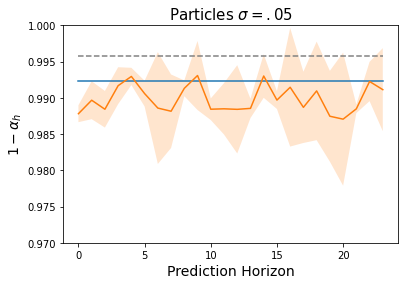
\includegraphics[width=\linewidth]{copula/figs/alphas/particle5.png}
  \label{fig:alpha-p2}
\end{subfigure}\\
\begin{subfigure}{.45\textwidth}
  \centering
  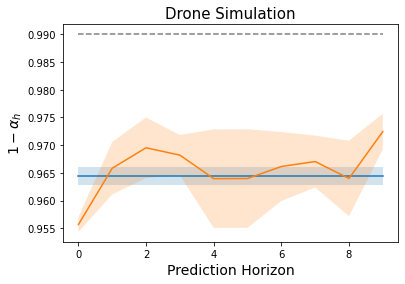
\includegraphics[width=\linewidth]{copula/figs/alphas/drone.png}
  \label{fig:alpha-drone}
\end{subfigure}%
\begin{subfigure}{.45\textwidth}
  \centering
  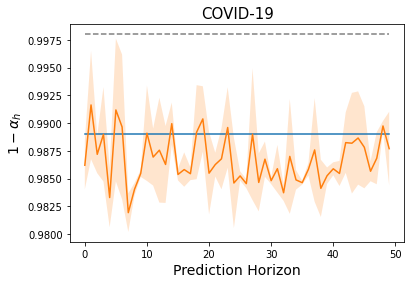
\includegraphics[width=\linewidth]{copula/figs/alphas/covid.png}
  \label{fig:alpha-covid}
\end{subfigure} \\
\begin{subfigure}{.46\textwidth}
  \centering
  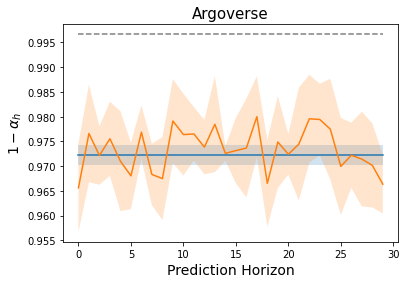
\includegraphics[width=\linewidth]{copula/figs/alphas/argo.png}
  \label{fig:alpha-argo}
\end{subfigure}
\begin{subfigure}{.45\textwidth}
  \centering
  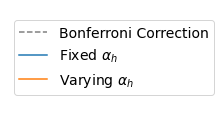
\includegraphics[width=0.6\linewidth]{copula/figs/alphas/labs.png}
  \label{fig:label}
\end{subfigure}
\caption{Comparison between dichotomy search for fixed $\alpha_h$ values (blue) and stochastic gradient search for varying $\alpha_h$ (blue) through timesteps. Shaded regions are the standard deviation of the values over 3 runs.} 
\label{fig:alpha}
\end{figure*}

\clearpage

\edit{
\subsection{Comparison to additional Baselines}}

We include a comparison to two additional simple UQ baselines on the particle simulation dataset. 

\textbf{L2-Conformal.} L2-Conformal uses the same underlying RNN forecaster as CF-RNN and Copula RNN.  We use that nonconformity score of the vector norm of all timesteps concatenated together $\| \hat{\textbf{y}}_{t+1:t+k} -\textbf{y}_{t+1:t+k} \|$ to perform ICP. As there are no analytic way to represent a $k \times d_y$-dimensional uncertainty region on 2-D space, we calculate the area and plot the region for L2 Conformal baseline with the maximum deviation at each timestep such that the vector norm still stays within range. 


\textbf{Direct Gaussian.} Direct Gaussian use the same model architecture and training hyperparameters, with the addition of a linear layer that outputs the variance for each timestep, and is optimized using negative log loss, a proper scoring rule for probabilistic forecasting. We obtain the area by analytically calculating the 90\% confidence interval for each variable.

Results in Table \ref{tab:partilel2} shows that L2-conformal produces inefficient confidence area, and directly outputting variance under-covers test data. These results align with previous findings and motivates our method, which is both more calibrated and sharper compared to these  baselines. We show a visualization in Figure \ref{fig:l2vis} to illustrate the different properties of the methods qualitatively.


\begin{table*}[h]
\centering
\begin{tabular}{ c | c c  | c c  |  } 
 \toprule
  & \multicolumn{2}{c}{Particle  ($\sigma=.01$)} & \multicolumn{2}{c}{Particle  ($\sigma=.05$)}\\
 \midrule
  Method & Coverage  (90\%) & Area  $\downarrow$ & Coverage  (90\%) & Area  $\downarrow$ \\
\midrule  
 L2-Conformal & $88.5 \pm 0.4$ & $7.21 \pm 0.35$  &  $89.7 \pm 0.6$  & $7.21 \pm 0.35$ \\
 Direct Gaussian & $11.9 \pm 0.09$ & $0.07 \pm 0.31$  & $0.0 \pm 0.0$ & $0.08 \pm 0.02$ \\
 CF-RNN &  $97.0 \pm 2.3$ & $3.13 \pm 3.24$ &  $97.0 \pm 2.3$ &  $5.79 \pm 0.51$ \\
 Copula-RNN & $\textbf{91.5} \pm 2.1$ & $\textbf{1.06} \pm 0.36$ & $\textbf{90.3} \pm 0.7$ & $\textbf{4.50} \pm 0.07$ \\
\bottomrule
 \end{tabular}
 \caption{ Comparison with two additional baselines on the particle dataset. }
\label{tab:partilel2}
 \end{table*}
 
 
\begin{figure}[h]
\centering
\begin{subfigure}[b]{0.45\linewidth}
  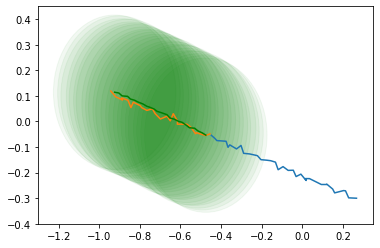
\includegraphics[width=\linewidth]{copula/figs/baselines2/l2.png}
  \caption{L2 Conformal}
  \label{fig:r1}
\end{subfigure}%
\begin{subfigure}[b]{0.45\linewidth}
  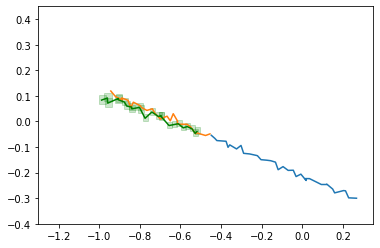
\includegraphics[width=\linewidth]{copula/figs/baselines2/gaussian.png}
  \caption{Direct RNN Gaussian}
  \label{fig:r2}
\end{subfigure}
\begin{subfigure}[b]{0.45\linewidth}
  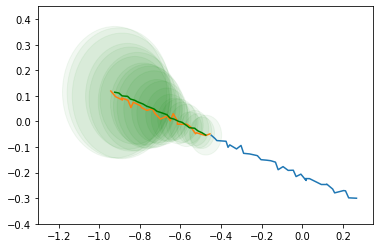
\includegraphics[width=\linewidth]{copula/figs/baselines2/cfrnn.png}
  \caption{CF-RNN}
  \label{fig:r3}
\end{subfigure}
\begin{subfigure}[b]{0.45\linewidth}
  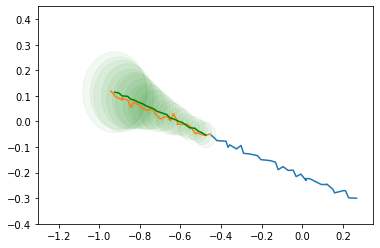
\includegraphics[width=\linewidth]{copula/figs/baselines2/copula.png}
  \caption{Copula-RNN}
  \label{fig:r4}
\end{subfigure}
\caption{ Visualization of on a sample from the Particle dataset's test set.  }
\label{fig:l2vis}
\end{figure}

% \begin{table*}[h]
% \centering
% \begin{tabular}{ c | c c   c c  |  } 
%  \toprule
%  Method & Coverage (90\%) & Area $\downarrow$ \\
% \midrule 
%  L2-Conformal & $88.5 \pm 0.4$ & $7.21 \pm 0.35$ \\
%  Direct Gaussian& $11.9 \pm 0.09$ & $0.07 \pm 0.31$ \\
%  CF-RNN &  $97.0 \pm 2.3$ & $3.13 \pm 3.24$ \\
%  Copula-RNN & $\textbf{91.5} \pm 2.1$ & $\textbf{1.06} \pm 0.36$ \\
% \bottomrule
%  \end{tabular}
%  \caption{ Particle dataset $\sigma = 0.01$, with confidence $1-\alpha = 0.9$  }
% \label{tab:partile1l2}
%  \end{table*}
 
 
 